\documentclass[11pt]{article}
\usepackage[utf8]{inputenc}	% Para caracteres en español
\usepackage{amsmath,amsthm,amsfonts,amssymb,amscd}
\usepackage{multirow,booktabs}
\usepackage[table]{xcolor}
\usepackage{fullpage}
\usepackage{lastpage}
\usepackage{enumitem}
\usepackage{fancyhdr}
\usepackage{mathrsfs}
\usepackage{wrapfig}
\usepackage{setspace}
\usepackage{calc}
\usepackage{multicol}
\usepackage{cancel}
\usepackage[retainorgcmds]{IEEEtrantools}
\usepackage[margin=3cm]{geometry}
\usepackage{amsmath}
\newlength{\tabcont}
\setlength{\parindent}{0.0in}
\setlength{\parskip}{0.05in}
\usepackage{empheq}
\usepackage{framed}
\usepackage[most]{tcolorbox}
\usepackage{xcolor}
\usepackage{pagecolor}
\usepackage{hyperref}
\usepackage{algorithm}
\usepackage{algpseudocode}
\algtext*{EndFor}
% \pagecolor{black}
% \color{white}

\colorlet{shadecolor}{blue!40}
\parindent 0in
\parskip 12pt
\geometry{margin=1in, headsep=0.25in}
\theoremstyle{definition}
\newtheorem{defn}{Definition}
\newtheorem{reg}{Rule}
\newtheorem{exer}{Exercise}
\newtheorem{note}{Note}

\newcommand{\XX}{\mathbf{X}}
\newcommand{\xx}{\mathbf{x}}
\newcommand{\zz}{\mathbf{z}}
\newcommand{\ZZ}{\mathbf{Z}}
\newcommand{\GG}{\mathbf{\Gamma}}
\newcommand{\rr}{\mathbf{r}}
\renewcommand{\AA}{\mathbf{A}}
\newcommand{\QQ}{\mathbf{Q}}
\newcommand{\RR}{\mathbf{R}}
\newcommand{\UU}{\mathbf{U}}
\newcommand{\uu}{\mathbf{u}}
\newcommand{\DD}{\mathbf{D}}
\newcommand{\VV}{\mathbf{V}}
\newcommand{\vv}{\mathbf{v}}
\renewcommand{\SS}{\mathbf{S}}
\newcommand{\HH}{\mathbf{H}}
\newcommand{\LL}{\mathbf{\Lambda}}
\newcommand{\YY}{\mathbf{Y}}
\newcommand{\yy}{\mathbf{y}}
\newcommand{\II}{\mathbf{I}}
\newcommand{\onevec}{\mathbf{1}}
\newcommand{\IID}{\textsf{IID}}
\newcommand{\ridge}{\textsf{ridge}}
\newcommand{\lasso}{\textsf{lasso}}
\newcommand{\ls}{\textsf{ls}}
\newcommand{\df}{\textsf{df}}

\newcommand{\Normal}[2]{\ensuremath{\mathcal N (#1, #2)}}
\newcommand{\ip}[2]{\ensuremath{\left\langle#1, #2\right\rangle}}

\DeclareMathOperator*{\argmax}{arg\,max}
\DeclareMathOperator*{\argmin}{arg\,min} \DeclareMathOperator*{\Cov}{Cov}
\DeclareMathOperator*{\EPE}{EPE} \DeclareMathOperator*{\Var}{Var}
\DeclareMathOperator*{\Bias}{Bias} \DeclareMathOperator*{\tr}{trace}
\DeclareMathOperator*{\RSS}{RSS} \DeclareMathOperator*{\WRSS}{WRSS}
\DeclareMathOperator*{\MSE}{MSE} \DeclareMathOperator*{\diag}{diag}

\begin{document}
\title{Chapter 3 Review Notes}

\thispagestyle{empty}

\begin{center}
	{\LARGE \bf Chapter 3 Lecture Notes}\\
	{\large Elements of Statistical Learning}
\end{center}

\section{Means and Variances}

\begin{shaded}
	\textbf{Important Properties of Estimators} \newline
	Let $x_1,\ldots,x_N$ be i.i.d. with mean $\mu$ and variance $\sigma^2$. Let
	$\hat \mu=E_i[x_i]$ and $\hat \sigma^2 = \frac{N}{N-1}E_i(x_i-\hat \mu)^2$ be
	the estimated mean and estimated variance respectively. Then $E[\hat\mu]=\mu$
	and $E[\hat\sigma^2]=\sigma^2$.
\end{shaded}

First, it is easy to show that $E[\hat \mu]=\mu$:
\begin{equation}
	\begin{split}
		E[\hat\mu] &= E[E_i[x_i]] \\
		&= E_i[E[x_i]] \\
		&= E_i[\mu] \\
		&= \mu.
	\end{split}
\end{equation}

Next, we know that
\begin{itemize}
	\item $\Var(c x)=c^2\Var(x)$
	\item $\Var(\sum x_i)=n\Var(x_i)=n\sigma^2$, since they are i.i.d..
	\item The above two, give us that $\Var[\hat\mu]=\frac{\sigma^2}{n}$. This
	      makes sense, the more data we have the closer we get to the mean, and so the
	      variance becomes smaller.
\end{itemize}

Using the above property, we can compute the expected estimated variance. First,
notice that
\begin{equation}
	\begin{split}
		E_i(x_i-\hat\mu)^2 &= E_i(x_i^2-2x_i\hat\mu+\hat\mu^2) \\
		&= E_i(x_i^2) - 2\hat\mu E_i(x_i) + \hat\mu^2 \\
		&= E_i(x_i^2) - \hat\mu^2.
	\end{split}
\end{equation}

Therefore, we compute $E(\hat\sigma^2)$ as follows:
\begin{equation}
	\begin{split}
		E(\hat\sigma^2) &= \frac{N}{N-1}E(E_i(x_i-\hat \mu)^2) \\
		&= \frac{N}{N-1}E(E_i(x_i^2) - \hat\mu^2) \\
		&= \frac{N}{N-1}\left[E(E_i(x_i^2)) - E(\hat\mu^2)\right] \\
		&= \frac{N}{N-1}\left[E_i(E(x_i^2)) - E(\hat\mu^2)\right] \\
		&= \frac{N}{N-1}\left[E_i(\sigma^2-\mu^2) - E(\hat\mu^2)\right] \\
		&= \frac{N}{N-1}\left[\sigma^2-\mu^2 - \Var\hat\mu+(E\hat\mu)^2\right] \\
		&= \frac{N}{N-1}\left[\sigma^2-\mu^2 - \sigma^2/N+\mu^2\right] \\
		&= \frac{N}{N-1}\frac{N-1}{N}\sigma^2 = \sigma^2.
	\end{split}
\end{equation}

\section{Estimated Values in Linear Regression}

\begin{shaded}
	\textbf{Important Properties of Estimators} \newline
	Suppose that the regression function $E[Y|X]=f(X)$ and that $\Var
		Y=\sigma^2$. Suppose also that $x_i$ are fixed, not random, and the only
	randomness is on the $y_i$. We compute the least squares as $\hat\beta =
		(\XX^T\XX)^{-1}\XX^T\yy$ and the estimated variance as
	$\hat\sigma^2=\frac{N}{N-p-1}E_i(y_i-\hat y_i)^2$. Then
	$\Var[\hat\beta]=(\XX^T\XX)^{-1}\sigma^2$ and $E[\hat\sigma^2]=\sigma^2$.
\end{shaded}

We first compute $\Var[\hat\beta]$. We have
\begin{equation}
	\begin{split}
		\Var[\hat\beta] &= \Var[(\XX^T\XX)^{-1}\XX^T\yy] \\
		&= (\XX^T\XX)^{-1}\XX^T \Var[\yy] \XX(\XX^T\XX)^{-1} \\
		&= (\XX^T\XX)^{-1}\XX^T \II_p\sigma^2 \XX(\XX^T\XX)^{-1} \\
		&= (\XX^T\XX)^{-1}\sigma^2.
	\end{split}
\end{equation}


\section{Important Distributions}

\subsection{Chi-squared}
Let $x_1,\ldots,x_n$ be \IID~ standard normal random variables
$x_i\sim\mathcal{N}(0,1)$ and let $\|x\|_2=nE_ix_i^2=\sum_i x_i^2$. Then
$$\|x\|_2\sim\chi_n^2.$$

Of course $\chi_n^2$ is always positive and drops similarly to how the normal
drops on its right.

Clearly, the same holds no matter whether the vector is free or bound. Hence, if
$x\sim\mathcal{N}(\mu,I_n)$, then $$\|x\|_2=\sum(x_i-\mu)^2\sim\chi_n^2$$ again.

Additionally, Cochran's theorem states that
$nE_i(x_i-E_ix_i)^2=\sum_i(x_i-\hat\mu)^2\sim\chi_{n-1}^2$. So, if we instead of
the real mean we use the estimated mean, we lose one degree of freedom.

Also, $(n-1)\hat\sigma^2\sim \sigma^2\chi_{n-1}^2$.

\subsection{$t$-distribution}
As before, let $x_1,\ldots,x_n\sim\Normal\mu{\sigma^2}$. We saw above that the
sample variance (a.k.a. unbiased variance estimation) is
$\hat\sigma^2=\frac{N}{N-1}E_i(x_i-\hat\mu)^2$. It holds that
\begin{equation}
	\frac{\hat\mu-\mu}{\sigma/\sqrt n}~\sim\Normal{0}{1}. \tag{See Wiki}
\end{equation}
However, if instead we use the sample variance, we get
\begin{equation}
	\frac{\hat\mu-\mu}{\hat\sigma/\sqrt n}~\sim t_{n-1}.
\end{equation}
Observe that both of the above quantities have distributions that do not depend
neither on $\mu$ nor on $\sigma$. However, specifically the second one has only
one unknown, the mean $\mu$. So we can use this distribution to derive
confidence intervals for $\mu$.

For example, we can make the null hypothesis that $\mu=\mu^*$ for some $\mu^*$.
If this is the case, then we expect the expression
\[\frac{\hat\mu-\mu^*}{\hat\sigma\sqrt{n}}\] to follow the
$t_{n-1}$-distribution which is almost the same as the normal distribution. But
note that we know all parameters of this expression so we can easily evaluate
it. If we get a value that is close to 0 then we accept the hypothesis,
otherwise we reject it.

\begin{shaded}
	\textbf{Hypothesis testing using the $t$-distribution} \newline
	As the sample size $n$ increases, the two distributions $\Normal 0 1$ and
	$t_{n-1}$ look very alike and $t_\infty=\Normal 0 1$. Especially the
	difference between their tail quantiles becomes negligible in $n$.
	This suggests an easy way to verify the null hypothesis that $\mu=0$. Simply
	take the quantity $\frac{\hat\mu}{\hat\sigma^2/\sqrt n}$ and check whether
	it is far from zero. The further from zero it is, the more likely that the
	null hypothesis does not hold and should be rejected.
\end{shaded}


\begin{defn}[$t$-distribution]
	Let $Z,V$ independent random variables, such that $Z\sim\Normal 0 1$ and
	$V\sim\chi_v^2$. Then
	\[T=\frac{Z}{\sqrt{V/v}}\sim t_v\]
\end{defn}

Student's $t$ looks like a normal distribution but pushed down.

\subsection{$F$-distribution}
My first observation is that the $F$ distribution is to the $t$-distribution
what the $\chi$-distribution is to the normal distribution. The $F$-distribution
has two degrees of freedom $d_1,d_2$ and we write $F_{d_1,d_2}$.


\begin{shaded}
	\textbf{Property of $\chi^2$ and $F$} \newline
	Suppose $X$ has a Student's $t$-distribution with degree of freedom $v$;
	i.e., $X\sim t_v$. Then $X^2\sim F_{1,v}$.
\end{shaded}

\begin{defn}
	Suppose $S_1\sim\chi_{d_1}^2$ and $S_2\sim\chi_{d_2}^2$ are two independent
	random variables. Then
	\[X=\frac{S_1/d_1}{S_2/d_2}\sim F_{d_1,d_2}.\]
\end{defn}
So it is the ratio of two independent appropriately scaled $\chi^2$ distributions.

Similarly to the chi-squared distribution, the $F$-distribution is always positive
and has a similar shape as the chi-squared.

\subsection{$Z$-score}
Let $X$ be a random variable with mean $\mu$ and variance $\sigma$. Let
$x\leftarrow X$, be a sample from this distribution. Then the $Z$-score of $x$
is the distance of $x$ from the mean, measured in standard deviations:
\[ z=\frac{x-\mu}{\sigma}.\]

Notice that if $x\sim\Normal{\mu}{\sigma^2}$, then $z\sim\Normal 0 1$; i.e., it
follows the standard normal distribution. This is called \emph{normalization} in
general. The goal is to use our samples to arrive to a \emph{pivotal quantity},
meaning a quantity whose distribution is known to us and is independent of the
parameters of the real distribution.

\paragraph{Example.} Suppose that $\hat x=\hat\mu=E_i x_i$ is the average (sample mean,
mean estimation) of the $x_i$s. We saw earlier that $E[\hat{x}]=\mu$. Moreover,
$\hat\sigma=\frac{N}{N-1}E_i(x_i-\hat\mu)^2$ is the sample variance such that
$E[\hat\sigma^2]=\sigma^2$. Then the Z-score of $\hat x$, is
\[z=\frac{\hat x-E[\hat x]}{\hat\sigma/\sqrt{N}}.\]
This follows the distribution $t_{N-1}$ as we saw.

\section{Applications to 3.2}
We have already seen that
\[\Var[\hat\beta]=(\XX^T\XX)^{-1}\sigma^2.\]

Moreover, similarly to how we computed the unbiased variance estimator above for
one dimension, here we have $p+1$ dimensions, and hence,
\[\hat\sigma^2=\frac{N}{N-p-1}E_i(\hat y_i-y_i)^2.\]

As before, $E[\hat\sigma^2]=\sigma^2$.

Now, let's additionally assume that the real model is linear; i.e.
$E[Y|X]=X^T\beta$ and $Y=X^T\beta+\varepsilon$, where
$\varepsilon\sim\Normal{0}{\sigma^2}$.

In this case, our beta estimator $\hat\beta$ is also normal:
\[\hat\beta\sim\Normal{\beta}{(\XX^T\XX)^{-1}\sigma^2}.\]

Moreover, $(N-p-1)\hat\sigma^2\sim\sigma^2\chi^2_{N-p-1}$ similarly to what we
had above but for more dimensions.

Also, $\Cov(\hat\beta,\hat\sigma^2)=0$. We define the Z-score of $\hat\beta_j$
as
\[z_j=\frac{\hat\beta_j-\beta_j}{\hat\sigma\sqrt{v_j}},\] where $v_j$ is the
$j$th diagonal element of $(\XX^T\XX)^{-1}$. Notice that in the above expression
the only unknown is $\beta_j$. So we can possibly plug different values until we
find an expression that is close to 0.

For example, if we make the null hypothesis that $\beta_j=0$, then $z_j\sim
	t_{N-p-1}$, which is almost the same as $\Normal 0 1$.

\subsection{Removing more variables}
Often, we may have a feeling that there is a group of coefficients that does not
affect the dependent variable. In this case, we can apply least squares
\emph{with} and \emph{without} this set of variables getting $\RSS_1$ and
$\RSS_0$ respectively. In this case, the F-statistic is:
\[F=\frac{(\RSS_0-\RSS_1)(p_1-p_0)}{\RSS_1/(N-p_1-1)},\] where $p_1+1$ is number
of parameters of the bigger model and $p_0+1$ is the number of parameters of the
smaller model. As we guess,
\[F\sim F_{p_1-p_0,N-p_1-1}.\] Again, the $F$-distribution is very similar to
the $\chi^2_{p_1-p_0}/(p_1-p_0)$ distribution at the tail quantiles. So the
further we are from zero, the more likely the larger model to be the correct
one.

\subsection{Confidence Intervals}
Finally, suppose that we have computed the pivotal quantity $z_j$ and got a
particular value. Now, since we know that the distribution of $z_j$ is very
close to the standard normal, we can get a confidence interval for $\beta_j$.

For example, suppose we want a 95\% confidence interval. Then, we look for a $c$
such that
\[\Pr[-c\le z_j\le c]=0.95,\]
which amounts to $c=1.96.$

We have
\begin{equation}
	\begin{split}
		-c\le \frac{\hat\beta_j-\beta_j}{\hat\sigma\sqrt{v_j}}\le c &\implies
		-c\hat\sigma\sqrt{v_j} \le \hat\beta_j-\beta_j \le c\hat\sigma\sqrt{v_j} \\
		&\implies -c\hat\sigma\sqrt{v_j}-\hat\beta_j \le -\beta_j \le c\hat\sigma\sqrt{v_j}-\hat\beta_j \\
		&\implies -c\hat\sigma\sqrt{v_j}+\hat\beta_j \le \beta_j \le c\hat\sigma\sqrt{v_j}+\hat\beta_j,
	\end{split}
\end{equation}
where $c$ is the 95\% percentile of the standard normal distribution. Hence,
with probability 95\%,
\[\beta_j\in
	(\hat\beta_j-c\hat\sigma\sqrt{v_j},\hat\beta_j+c\hat\sigma\sqrt{v_j}),\] where
$\hat\sigma\sqrt{v_j}=\mathrm{se}(\hat\beta_j)$ is the standard error of
$\hat\beta_j$. By approximating $c=2$, we get the standard practice of reporting
$\hat\beta_j\pm \mathrm{se}(\hat\beta_j)$ as the 95\% confidence interval.

\subsection{Reproducing Correlation Matrix}
By running the python script \texttt{prostate-data/correlation.py}, we get
	{\footnotesize
		\begin{verbatim}
                                 Correlation Matrix
========================================================================================
           cavol  lweight      age     lbph      svi      lcp  gleason    pgg45     lpsa
lcavol   1.00000  0.30023  0.28632  0.06317  0.59295  0.69204  0.42641  0.48316  0.73316
lweight  0.30023  1.00000  0.31672  0.43704  0.18105  0.15683  0.02356  0.07417  0.48522
age      0.28632  0.31672  1.00000  0.28735  0.12890  0.17295  0.36592  0.27581  0.22764
lbph     0.06317  0.43704  0.28735  1.00000 -0.13915 -0.08853  0.03299 -0.03040  0.26294
svi      0.59295  0.18105  0.12890 -0.13915  1.00000  0.67124  0.30688  0.48136  0.55689
lcp      0.69204  0.15683  0.17295 -0.08853  0.67124  1.00000  0.47644  0.66253  0.48920
gleason  0.42641  0.02356  0.36592  0.03299  0.30688  0.47644  1.00000  0.75706  0.34243
pgg45    0.48316  0.07417  0.27581 -0.03040  0.48136  0.66253  0.75706  1.00000  0.44805
lpsa     0.73316  0.48522  0.22764  0.26294  0.55689  0.48920  0.34243  0.44805  1.00000
                            OLS Regression Results                            
==============================================================================
Dep. Variable:                   lpsa   R-squared:                       0.694
Model:                            OLS   Adj. R-squared:                  0.652
Method:                 Least Squares   F-statistic:                     16.47
Date:                Fri, 01 Apr 2022   Prob (F-statistic):           2.04e-12
Time:                        20:36:00   Log-Likelihood:                -55.359
No. Observations:                  67   AIC:                             128.7
Df Residuals:                      58   BIC:                             148.6
Df Model:                           8                                         
Covariance Type:            nonrobust                                         
==============================================================================
                 coef    std err          t      P>|t|      [0.025      0.975]
------------------------------------------------------------------------------
const       1.527e-16      0.073    2.1e-15      1.000      -0.145       0.145
lcavol         0.5931      0.111      5.366      0.000       0.372       0.814
lweight        0.2423      0.088      2.751      0.008       0.066       0.419
age           -0.1180      0.085     -1.396      0.168      -0.287       0.051
lbph           0.1755      0.085      2.056      0.044       0.005       0.346
svi            0.2563      0.104      2.469      0.017       0.049       0.464
lcp           -0.2393      0.128     -1.867      0.067      -0.496       0.017
gleason       -0.0173      0.118     -0.147      0.884      -0.254       0.219
pgg45          0.2296      0.132      1.738      0.088      -0.035       0.494
==============================================================================
Omnibus:                        0.825   Durbin-Watson:                   1.690
Prob(Omnibus):                  0.662   Jarque-Bera (JB):                0.389
Skew:                          -0.164   Prob(JB):                        0.823
Kurtosis:                       3.178   Cond. No.                         4.44
==============================================================================

Notes:
[1] Standard Errors assume that the covariance matrix of the errors is correctly specified.

<F test: F=1.6697548846375199, p=0.16933707265225223, df_denom=58, df_num=4>
\end{verbatim}
	}

In the above, the $z$-score is denoted by \texttt t and measures the effect of
dropping the variable from the model. An absolute value greater than $2$, means
that with high probability this variable is significant.

\section{Shrinkage}
Dropping predictors is only one way we can potentially reduce the variance at
the cost of introducing bias. By dropping some parameters we also get the
advantage of having a smaller and more intuitive model. However, the downside of
best subset selection is that it is a discrete process so it does not usually
behave well.

Ridge regression shrinks the coefficients of the linear regression but in a
``homogeneous'' way. It does not allow for a huge shrinkage in one coefficient
but no shrinkage in another. How can we enforce this?

\begin{itemize}
	\item Ridge regression. Here, we impose a universal penalty defined via
	      the complexity parameter $\lambda$ and hence we try to minimize the expression:
	      \[\RSS^\ridge(\lambda,\beta)=\sum_{i\in[N]}\left(y_i-\beta_0-\sum_{j\in[p]}x_{i,j}\beta_j\right)^2
		      + \lambda\sum_{j\in[p]}\beta_j^2\]

	\item The lasso. Here we use a different norm and we have:
	      \[\RSS^\lasso(\lambda,\beta)=\sum_{i\in[N]}\left(y_i-\beta_0-\sum_{j\in[p]}x_{i,j}\beta_j\right)^2
		      + \lambda\sum_{j\in[p]}|\beta_j|\]

	\item In general, we could have any norm, and so we would get
	      \[\RSS^q(\lambda,\beta)=\RSS(\beta) + \lambda \|\beta\|_q,\] where
	      $\RSS(\beta)=(\yy-\XX\beta)^T(\yy-\XX\beta)$.
\end{itemize}
Notice that now, one cannot have too ``long'' coefficients since this would make
the $\RSS$ considerably large. In other words, these new metrics, enforce
picking small coefficients. This is not the case necessarily in a linear
regression model since one could have a very large positive coefficient
$\beta_i$ and a very large negative coefficient $\beta_j$. These, would cancel
each other in $\RSS$ and could give us a small error, yet a very large variance.
On the other hand, they would not cancel each other in these expanded versions
since we add up their absolute values.

\paragraph{Notes}
\begin{itemize}
	\item Ridge regression is not equivariant under scaling of inputs.
	\item It is normal to first standardize the inputs before applying ridge
	      regression
	\item We need to omit the intercept $\beta_0$ from the procedure. If we
	      don't, then shifting each target $y_i$ by a constant $c$ does not simply
	      shift the predictions by $c$. In other words, if we include $\beta_0$, then
	      the procedure would depend on the origin chosen for $Y$. I don't see why
	      this is bad. It is not a linear model if the first case.
	\item Assuming we omit $\beta_0$ from the process, we work as follows:
	      \begin{enumerate}
		      \item Set $x_{i,j}=x_{i,j}-\overline x_j$, $i\in[N],j\in[p]$. These are
		            called the \emph{centered} inputs.
		      \item Set $\beta_0=\overline y$
		      \item Run ridge regression without intercept, where $\XX$ has $p$
		            columns.
	      \end{enumerate}
\end{itemize}
Now we just need to find
\[\argmin_\beta \left[(\yy-\XX\beta)^T(\yy-\XX\beta) + \lambda\beta^T\beta\right],\]
where $\XX$ has $p$ columns.

\subsection{Ridge Interpretation as the Mode of a Distribution}
Suppose that $y\sim \Normal{\beta_0+x^T\beta}{\sigma^2}$ and
$\beta\sim\Normal{0}{\tau^2 \II}$. Now, given $N$ samples $(x_i,y_i)_{i\in[N]}$,
what is the conditional distribution of $\beta$? Notice that there is a
dependency between the samples and $\beta$, therefore, the distribution of
$\beta$ given the samples is not necessarily the same as original distribution.
It can be shown that
\[-\log f(\beta|(x_i,y_i)_{i\in[N]})=\RSS^\lasso(\lambda,\beta),\] where
$\lambda=\sigma^2/\tau^2$ and $f(\beta)$ is the conditional probability density
function of $\beta$, given the samples.

Now, by definition,
\[\argmax_\beta\RSS^\lasso(\lambda,\beta) = \text{mode}(f).\]

\subsection{Solution of Ridge Regression}
Minimizing the criterion $\RSS(\lambda,\beta) = \RSS(\beta) + \lambda\|\beta\|_2
	= (\yy-\XX\beta)^T(\yy-\XX\beta)+\lambda\beta^T\beta$, gives us the solution
\[
	\hat\beta^\ridge = (\XX^T\XX+\lambda \II)^{-1}\XX^T\yy.\]
Compare this with the least squares solution
\[\hat\beta = (\XX^T\XX)^{-1}\XX^T\yy.\]

\paragraph{Observation.} Note that in ridge regression, as with least squares,
it is very rare that a coefficient will be zero. On the other hand, we would be
interested in being able to compare the ridge solution with the subset selection
solution. This becomes possible using the effective degrees of freedom:
\[\df(\lambda)=\tr[\XX(\XX^T\XX+\lambda\II)^{-1}\XX^T]=\sum_{j=1}^p\frac{d_j^2}{d_j^2+\lambda}.\]

Notice that this value is at most $p$ and if $\lambda=0$, we get the standard
least squares solution and $\df(0)=p$. By setting some of the coefficients to 0
in subset selection, we get a smaller value.

\begin{center}
	\emph{Assuming that the response has higher variance along the directions of
		inputs with higher variance, Ridge regression performs better.}
\end{center}


\section{Important Matrix Decompositions}

\subsection{Eigendecomposition}
Let $\AA$ be an $N\times N$ matrix with eigenvectors $q_1,\ldots,d_N$ and
eigenvalues $\lambda_1,\ldots,\lambda_N$. Then we know that
\begin{equation}
	\begin{split}
		\AA q_i &=  q_i\lambda_i \\
		\implies\AA\QQ &= \QQ\LL \\
		\implies\AA &= \QQ\LL\QQ^{-1}\text{ and }\AA^{-1}=\QQ\LL^{-1}\QQ^{-1}
	\end{split}
\end{equation}
where $\QQ=[q_1,\ldots,q_N]$ is an $N\times N$ matrix whose $i$th column is
$q_i$. So if we know $Q$ and $Q^{-1}$, we can just invert $\LL$ and since
$\diag^{-1}{(\lambda_1,\ldots,\lambda_N)}=\diag(1/\lambda_1,\ldots,1/\lambda_N)$,
this is easy to calculate.

\subsection{Singular Value Decomposition}
SVD is the generalization of eigendecomposition for matrices that are not
square. If $\XX$ is an $N\times p$ matrix, then it can be written as
\[\XX = \UU \DD \VV^T,\]
where
\begin{itemize}
	\item $\UU=[u_1,\ldots,u_p]$ is $N\times p$. Its columns span the
	      columnspace of $\XX$. It is orthogonal, meaning $\UU^T=\UU^{-1}$, and more
	      generally, it is unitary, if complex ($\UU^*=\UU^{-1}$).
	\item $\VV=[v_1,\ldots,v_p]$ is $p\times p$. Its columns span the rowspace
	      of $\XX$. Similarly, it is also unitary: $\VV^T=\VV^{-1}$.
	\item $\DD=\diag{(d_1,\ldots,d_p)}$, such that $d_1\ge d_2\ldots\ge d_p\ge
		      0$, called the singular values of $\XX$.
\end{itemize}
We can rewrite $\XX$ as
\[\XX=\sum_{j\in[p]}d_iu_iv_i^T.\,\]
which shows that $\XX$ can be written as the sum of $p$ rank-1 matrices.

More intuition about SVD can be found
\href{https://stats.stackexchange.com/questions/177102/what-is-the-intuition-behind-svd}{here}.

We see that
\[\XX^T\XX=\VV\DD^T\UU^T\UU\DD\VV^T=\VV(\DD^T\DD)\VV^T\]
\[\XX\XX^T=\UU\DD\VV^T\VV\DD^T\UU^T=\UU(\DD\DD^T)\UU^T\]

So these are the eigendecompositions of $\XX^T\XX$ and $\XX\XX^T$ respectively.

\subsubsection{Applying SVD to Least Squares and Ridge Regression}

\paragraph{Least Squares.} The least squares fitted vector can be written as
\begin{equation}
	\begin{split}
		\hat\yy^\ls &= \XX\hat\beta^\ls \\
		&= \XX(\XX^T\XX)^{-1}\XX^T\yy \\
		&= \UU\UU^T\yy.
	\end{split}
\end{equation}
In other words, $\UU\UU^T$ is another hat matrix.

\paragraph{Ridge.} Now for ridge regression, the fitted vector can be written as
\begin{equation}
	\begin{split}
		\hat\yy^\ridge &= \XX\hat\beta^\ridge \\
		&= \UU\DD(\DD\DD^T+\lambda\II)^{-1}\DD\UU^T\yy \\
		&= \sum_{j=1}^p\uu_j\frac{d_j^2}{d_j^2+\lambda}\uu_j^T\yy,
	\end{split}
\end{equation}
where $\uu_j$ are the column vectors of $\UU$.

We see that ridge regression, like linear regression computes the coordinates of
$\yy$ with respect to the orthonormal basis $\UU$. The difference is that ridge
regression also shrinks these coordinates by the fraction above.

\subsection{QR Decomposition}
The QR decomposition states that any real $N\times p$ matrix $\XX$ can be written as
\[\XX=\QQ\RR,\]
where
\begin{itemize}
	\item $\QQ$ is an $N\times p$ orthogonal matrix, meaning $\QQ^T=\QQ^{-1}$.
	\item $\RR$ is a $p\times p$ upper triangular matrix.
\end{itemize}

We know of three ways to create the QR decomposition: (a) Gram-Schmidt, (b)
Householder reflections, which is very similar to Grover's algorithm, and (c)
Givens rotations.

\section{Intuition of Linear Regression}
Linear regression is defined as
\[\hat\beta=(\XX^T\XX)^{-1}\XX^T y.\] However, this does not give us any
intuition other than it being the argmax of the residual sum of squares. Here we
start with the basics, and we first consider the scenario of univariate
regression.

Suppose that we have only one variable and $N$ samples, hence
$\xx=\XX\in\mathbb{R}^{N\times 1}$ where $\xx=[x_1,\ldots,x_N]^T$. As always,
suppose $\yy=[y_1,\ldots,y_N]^T$. What is the least squares estimate in this
case? Minimizing the RSS, we get
\[\hat\beta=\frac{\sum_{i=1}^N x_iy_i}{\sum_{i=1}^N
		x_ix_i}=\frac{\ip\xx\yy}{\ip\xx\xx},\]

called the \emph{univariate estimate}. Since
$\mathrm{proj}_\xx\yy=\hat\beta\xx$, we see that $\hat\beta$ corresponds to the
length of the projection of $\yy$ on $\xx$ as a fraction of the length of $\xx$.

Moreover, letting $r_i=y_i-x_i\hat\beta$, we get
$\rr=\yy-\xx\hat\beta=\yy-\mathrm{proj}_\xx\yy$. In other words, the residuals
are just the vectors that need to be added to the projection to get $\yy$.
Observe that the residual $\rr$ from regressing $\yy$ on $\xx$ is orthogonal to
$\xx$, i.e., $\ip\rr\xx=0$.

\subsection{Orthogonal Inputs}
Suppose now that we have $p$ variables and hence $\XX=[\xx_1,\ldots,\xx_p]$,
with $\xx_i\in\mathbb{R}^N$. Suppose, moreover, that $\ip{\xx_j}{\xx_k}=0$ for
any $j\ne k$. Then we can see that each $\hat\beta_j$ depends only on $\xx_j$
and $\yy$, and in particular,
\[\hat\beta_j=\frac{\ip{\xx_j}\yy}{\ip{\xx_j}{\xx_j}}.\] So for each variable,
the corresponding estimate is independent of the other variables.

\subsection{General Inputs}
In general, the inputs are rarely orthogonal and therefore we cannot conclude
that $\hat\beta_j$ depends only on $\xx_j$. However, if we first orthogonalize
the inputs, then this idea carries over. We apply this orthogonalization in the
next two subsections.

\subsubsection{Univariate Regression with Intercept}
Consider a single variable again, so $\xx=[x_1,\ldots,x_N]^T$ but that we
additionally have an intercept $\hat\beta_0$ that we want to compute. Denote
$\xx_0=[1,\ldots,1]^T=\onevec_N$. Then, if we regress $\xx$ on $\xx_0$, we get
coefficient
\[\hat\beta_0=\frac{\ip{\xx_0}\xx}{\ip{\xx_0}{\xx_0}}=\frac{\sum x_i}{N}=E_ix_i=\overline{x}\]
and residual
\[\zz=\xx-\overline{x}\xx_0=\xx-\overline{x}\onevec.\]

Finally, to compute $\hat\beta_1$, we regress $\yy$ on $\zz$ and we get
\[\hat\beta_1=\frac{\ip\yy\zz}{\ip\zz\zz}=\frac{\ip\yy{\xx-\overline{x}\onevec}}{\ip{\xx-\overline{x}\onevec}{\xx-\overline{x}\onevec}}\]

So what we did was
\begin{enumerate}
	\item We adjust $\xx$ for $\onevec$, getting a coefficient $\hat\beta_0$ and
	      residual $\zz=\xx-\hat\beta_0\onevec$.
	\item We adjust $\yy$ for $\zz$ getting a coefficient $\hat\beta_1$ and
	      residual $\zz'=\yy-\hat\beta_1\zz$ (although we are not interested in the
	      final residual).
\end{enumerate}

\subsubsection{Many Variables}
So, now we can easily generalize.
\begin{algorithm}
	\caption{Regression by Succesive orthogonalization}\label{alg:Gram-Schmidt}
	\begin{algorithmic}
		\State $\xx_0=\zz_0=\onevec$
		\For{$j=1,\ldots,p$}
		\State Regress $\xx_i$ on all \emph{previous} $\zz_0,\ldots,\zz_{j-1}$
		to get coefficients $\hat\gamma_{0,j},\ldots,\hat\gamma_{j-1,j}$ and
		residual $\zz_j=\xx_j-\sum \gamma_{\ell,j}\zz_\ell$.
		\EndFor
		\State Regress $\yy$ on $\zz_p$ to get coefficient $\hat\beta_p$.
	\end{algorithmic}
\end{algorithm}

Notice that since all $\zz_j$ are orthogonal to each other, they form a basis
for the column space of $\XX$.

So overall, if we want the estimate $\hat\beta_j$, all we need to do is adjust
$\xx_j$ for $\xx_1,\ldots,\xx_{j-1},\xx_{j+1},\ldots,\xx_p$ getting residual
$\zz_j$, and then adjust $\yy$ for $\zz_j$.

\begin{shaded}
	\textbf{Intuition on coefficients} \newline
	The coefficient $\hat\beta_j$ represents the information of $\yy$ that
	depends of $\xx_j$, after $\xx_j$ has been adjusted for the remaining
	predictors.
\end{shaded}

Before, we saw that the variance-covariance matrix of the estimates is
\[\Var{[\hat\beta]}=(\XX^T\XX)^{-1}\sigma^2.\]
An alternative formular of the estimates variance is
\[\Var{[\hat\beta_j]}=\frac{\sigma^2}{\ip{\zz_j}{\zz_j}}.\]

Notice that if $\xx_j$ is very correlated with one or more other parameters,
then the corresponding residual $\zz_j$ will be very short. In this case, it
would be better to use the Z-score to remove it. Moreover, notice that in this
case, its variance will be huge.

\subsubsection{Another interpretation of QR Decomposition}
If we set $\ZZ=[\zz_1,\ldots,\zz_p]$ and $\GG$ as the matrix with elements
$\hat\gamma_{\ell,j}$, then we get
\[\XX=\ZZ\GG,\] where $\GG$ is upper triangular. Notice that although the
columns of $\ZZ$ are orthogonal, they are not also orthonormal. By dividing each
row with its length $\|\zz_i\|$ we can make them orthonormal. This is expressed
by introducing the matrix $\DD=\diag(\|\zz_0\|,\ldots,\|\zz_p\|)$ and having
\[\QQ = \ZZ\DD^{-1}\] and \[\RR=\DD\GG.\] Now, $\QQ$ is orthonormal, and so,
$\QQ^T\QQ=\II$ and $\RR$ remains upper triangular.

Notice that now, we can get another least squares solution by setting to zero
the first derivative
\begin{equation}
	\begin{split}
		\XX^T(\yy-\XX\beta) &= \RR^T\QQ^T(\yy-\QQ\RR\beta) \\
		&= \RR^T\QQ^T\yy - \RR^T\RR\beta.
	\end{split}
\end{equation}
We get
\[\RR^T\RR\beta = \RR^T\QQ^T\yy\implies \RR\beta = \QQ^T\yy\implies \hat\beta =
	\RR^{-1}\QQ^T\yy.\] Of course, this assumes that $\RR^T$ (and therefore $\RR$)
is invertible. Moreover, the hat matrix can now be computed as
\[\hat\yy=\XX\hat\beta=\XX\RR^{-1}\QQ^T\yy=\QQ\RR\RR^{-1}\QQ^T\yy=\QQ\QQ^T\yy =
	\HH\yy.\]


\section{Principal Components}
Let $\XX=\UU\DD\VV^T$ be the SVD decomposition of $\XX$. The eigendecomposition
of $\XX^T\XX$ is
\[\XX^T\XX=\VV\DD^T\DD\VV^T,\] so the column vectors of $\VV$ are the
eigenvectors of $\XX^T\XX$ and the corresponding eigenvalues are the elements of
the diagonal of $\DD^T\DD$. The columns $\vv_j$ of $\VV$ are also called the
principal components \emph{directions} of $\XX$. The corresponding principal
components of $\XX$ are then $\zz_j=\XX\vv_j=\uu_jd_j$, where $d_j$ are the
singular values of $\XX$. Moreover, $\uu_j$ are the normalized principal
components.

Notice that up to a scalar $N$, the above is also the sample covariance matrix.
In other words,
\[\SS=\frac{\XX^T\XX}{N}.\]

\paragraph{Takeaways.}
\begin{center}
	\emph{ The small singular values correspond to directions in the column
		space of $\XX$ having small variance. Ridge regression shrinks these
		directions the most.}
\end{center}

\begin{center}
	\emph{ Conversely, the eigenvectors with the largest eigenvalues of the
		(sample) covariance matrix correspond the directions along which $\XX$ has
		the maximum variance.}
\end{center}

\section{A Few Notes on the Lasso}
The lasso solution is:
\[
	\hat\beta^\lasso=\argmin_\beta \left(\frac{1}{2}\sum_{i=1}^N \left(y_i - \beta_0 - \sum_{j=1}^p x_{ij}\beta_j\right)^2 + \lambda\sum_{j=1}^p|\beta_j|\right)\]

Equivalently, it is the solution to the following quadratic programming problem:

\begin{equation}
	\begin{split}
		\hat\beta^\lasso = &\argmin_\beta \sum_{i=1}^N \left(y_i-\beta_0-\sum_{j=1}^px_{ij}\beta_j\right)^2 \\
		& \text{subject to} \sum_{j=1}^p|\beta_j| \le t.
	\end{split}
\end{equation}
There is a one-to-one correspondence between $\lambda$ and $t$.

Contrary to ridge regression, there is no analytical solution. Nonetheless, it
can be found algorithmically with around the same complexity as ridge. This is
interesting because the ridge solution can be computed by just multiplying some
matrices (or maybe by using a modification of Gram-Schmidt?). So my guess is
that the ridge solution can be computed in around $O(N^3)$ time.

If $\lambda$ is sufficiently small, some of the coefficients will be 0 but it is
not clear why. For an intuition, see
\href{https://stats.stackexchange.com/questions/74542/why-does-the-lasso-provide-variable-selection}{here}.

Let $\hat\beta^\ls$ be the least squares coefficients. If
$t>\|\hat\beta^\ls\|_1$, then $t$ is too large and the solution gives again the
least squares coefficients. Intuitively, if $t>\|\hat\beta^\ls\|_1/2$, then the
lasso solution is around half the least squares solution; i.e.,
$\|\hat\beta^\lasso\|_1 \approx \|\hat\beta^\ls\|_1/2$. This is interesting. Can
we prove this?

\section{Subset Selection vs Ridge vs Lasso}
Let $\hat\beta$ be the least squares solution and assume that the input $\XX$ is
orthonormal. Then
\begin{itemize}
	\item $M$-subset selection keeps the $M$ largest coeefficients and zeroizes
	      all the rest.
	\item $\lambda$-ridge regression, shrinks by a factor of $\lambda$:
	      $\hat\beta_j^\ridge= \hat\beta_j/(1+\lambda)$.
	\item $\lambda$-lasso, shortens $\hat\beta$ by
	      $\lambda$ and zeroizes it if it is already short.
\end{itemize}

\begin{figure}[h]
	\centering
	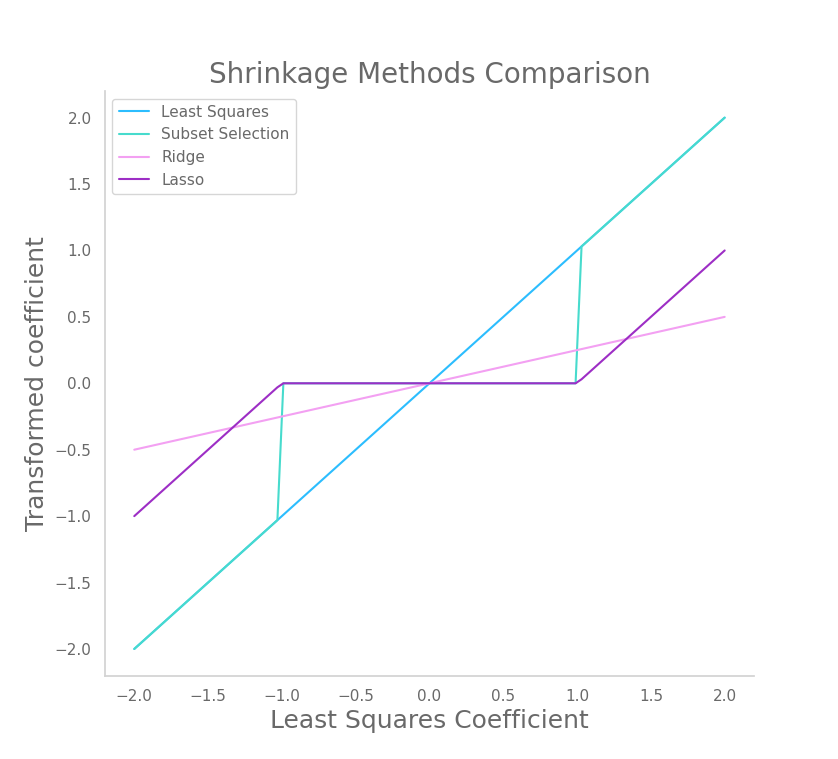
\includegraphics[width=10cm]{shrinkage-comparison.png}
\end{figure}
We see that the Lasso behaves like subset selection but additionally it shrinks
the larger coefficients.

\end{document}